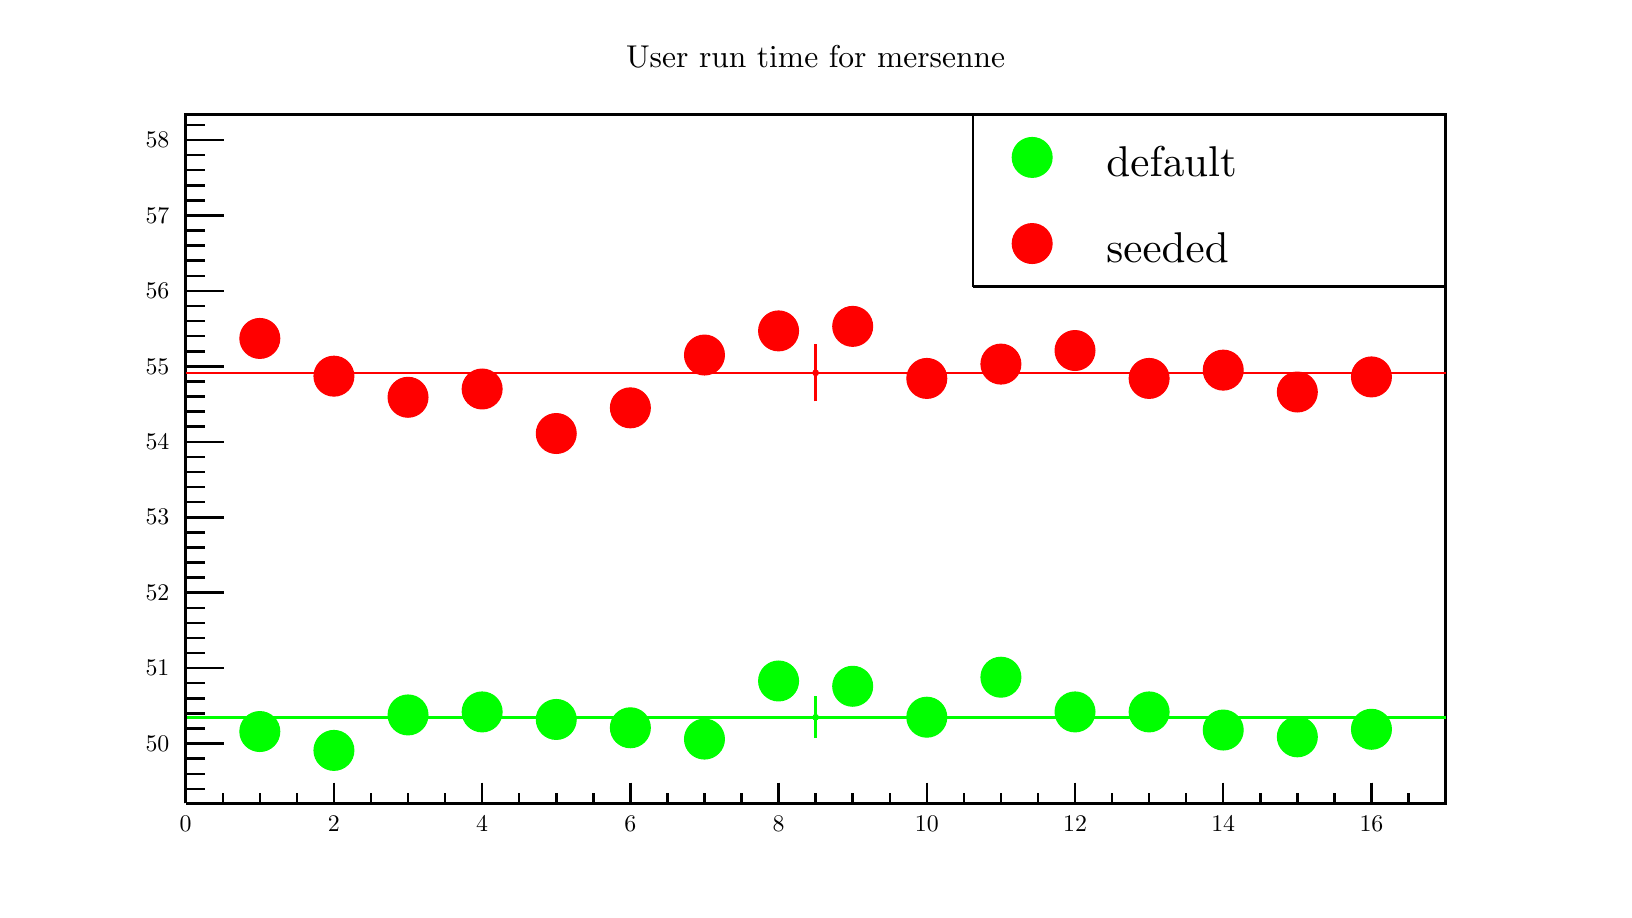
\begin{tikzpicture}
\pgfdeclareplotmark{cross} {
\pgfpathmoveto{\pgfpoint{-0.3\pgfplotmarksize}{\pgfplotmarksize}}
\pgfpathlineto{\pgfpoint{+0.3\pgfplotmarksize}{\pgfplotmarksize}}
\pgfpathlineto{\pgfpoint{+0.3\pgfplotmarksize}{0.3\pgfplotmarksize}}
\pgfpathlineto{\pgfpoint{+1\pgfplotmarksize}{0.3\pgfplotmarksize}}
\pgfpathlineto{\pgfpoint{+1\pgfplotmarksize}{-0.3\pgfplotmarksize}}
\pgfpathlineto{\pgfpoint{+0.3\pgfplotmarksize}{-0.3\pgfplotmarksize}}
\pgfpathlineto{\pgfpoint{+0.3\pgfplotmarksize}{-1.\pgfplotmarksize}}
\pgfpathlineto{\pgfpoint{-0.3\pgfplotmarksize}{-1.\pgfplotmarksize}}
\pgfpathlineto{\pgfpoint{-0.3\pgfplotmarksize}{-0.3\pgfplotmarksize}}
\pgfpathlineto{\pgfpoint{-1.\pgfplotmarksize}{-0.3\pgfplotmarksize}}
\pgfpathlineto{\pgfpoint{-1.\pgfplotmarksize}{0.3\pgfplotmarksize}}
\pgfpathlineto{\pgfpoint{-0.3\pgfplotmarksize}{0.3\pgfplotmarksize}}
\pgfpathclose
\pgfusepathqstroke
}
\pgfdeclareplotmark{cross*} {
\pgfpathmoveto{\pgfpoint{-0.3\pgfplotmarksize}{\pgfplotmarksize}}
\pgfpathlineto{\pgfpoint{+0.3\pgfplotmarksize}{\pgfplotmarksize}}
\pgfpathlineto{\pgfpoint{+0.3\pgfplotmarksize}{0.3\pgfplotmarksize}}
\pgfpathlineto{\pgfpoint{+1\pgfplotmarksize}{0.3\pgfplotmarksize}}
\pgfpathlineto{\pgfpoint{+1\pgfplotmarksize}{-0.3\pgfplotmarksize}}
\pgfpathlineto{\pgfpoint{+0.3\pgfplotmarksize}{-0.3\pgfplotmarksize}}
\pgfpathlineto{\pgfpoint{+0.3\pgfplotmarksize}{-1.\pgfplotmarksize}}
\pgfpathlineto{\pgfpoint{-0.3\pgfplotmarksize}{-1.\pgfplotmarksize}}
\pgfpathlineto{\pgfpoint{-0.3\pgfplotmarksize}{-0.3\pgfplotmarksize}}
\pgfpathlineto{\pgfpoint{-1.\pgfplotmarksize}{-0.3\pgfplotmarksize}}
\pgfpathlineto{\pgfpoint{-1.\pgfplotmarksize}{0.3\pgfplotmarksize}}
\pgfpathlineto{\pgfpoint{-0.3\pgfplotmarksize}{0.3\pgfplotmarksize}}
\pgfpathclose
\pgfusepathqfillstroke
}
\pgfdeclareplotmark{newstar} {
\pgfpathmoveto{\pgfqpoint{0pt}{\pgfplotmarksize}}
\pgfpathlineto{\pgfqpointpolar{44}{0.5\pgfplotmarksize}}
\pgfpathlineto{\pgfqpointpolar{18}{\pgfplotmarksize}}
\pgfpathlineto{\pgfqpointpolar{-20}{0.5\pgfplotmarksize}}
\pgfpathlineto{\pgfqpointpolar{-54}{\pgfplotmarksize}}
\pgfpathlineto{\pgfqpointpolar{-90}{0.5\pgfplotmarksize}}
\pgfpathlineto{\pgfqpointpolar{234}{\pgfplotmarksize}}
\pgfpathlineto{\pgfqpointpolar{198}{0.5\pgfplotmarksize}}
\pgfpathlineto{\pgfqpointpolar{162}{\pgfplotmarksize}}
\pgfpathlineto{\pgfqpointpolar{134}{0.5\pgfplotmarksize}}
\pgfpathclose
\pgfusepathqstroke
}
\pgfdeclareplotmark{newstar*} {
\pgfpathmoveto{\pgfqpoint{0pt}{\pgfplotmarksize}}
\pgfpathlineto{\pgfqpointpolar{44}{0.5\pgfplotmarksize}}
\pgfpathlineto{\pgfqpointpolar{18}{\pgfplotmarksize}}
\pgfpathlineto{\pgfqpointpolar{-20}{0.5\pgfplotmarksize}}
\pgfpathlineto{\pgfqpointpolar{-54}{\pgfplotmarksize}}
\pgfpathlineto{\pgfqpointpolar{-90}{0.5\pgfplotmarksize}}
\pgfpathlineto{\pgfqpointpolar{234}{\pgfplotmarksize}}
\pgfpathlineto{\pgfqpointpolar{198}{0.5\pgfplotmarksize}}
\pgfpathlineto{\pgfqpointpolar{162}{\pgfplotmarksize}}
\pgfpathlineto{\pgfqpointpolar{134}{0.5\pgfplotmarksize}}
\pgfpathclose
\pgfusepathqfillstroke
}
\definecolor{c}{rgb}{1,1,1};
\draw [color=c, fill=c] (0,0) rectangle (20,10.9387);
\draw [color=c, fill=c] (2,1.09387) rectangle (18,9.84481);
\definecolor{c}{rgb}{0,0,0};
\draw [c,line width=0.9] (2,1.09387) -- (2,9.84481) -- (18,9.84481) -- (18,1.09387) -- (2,1.09387);
\definecolor{c}{rgb}{1,1,1};
\draw [color=c, fill=c] (2,1.09387) rectangle (18,9.84481);
\definecolor{c}{rgb}{0,0,0};
\draw [c,line width=0.9] (2,1.09387) -- (2,9.84481) -- (18,9.84481) -- (18,1.09387) -- (2,1.09387);
\definecolor{c}{rgb}{0,1,0};
\draw [c,line width=0.9] (10,1.92196) -- (10,2.18744);
\draw [c,line width=0.9] (10,2.18744) -- (10,2.45291);
\draw [c,line width=0.9] (2,2.18744) -- (10,2.18744);
\draw [c,line width=0.9] (10,2.18744) -- (18,2.18744);
\foreach \P in {(10,2.18744)}{\draw[mark options={color=c,fill=c},mark size=2.402402pt,mark=*,mark size=1pt] plot coordinates {\P};}
\definecolor{c}{rgb}{0,0,0};
\draw [c,line width=0.9] (2,1.09387) -- (18,1.09387);
\draw [c,line width=0.9] (2,1.3564) -- (2,1.09387);
\draw [c,line width=0.9] (2.47059,1.22513) -- (2.47059,1.09387);
\draw [c,line width=0.9] (2.94118,1.22513) -- (2.94118,1.09387);
\draw [c,line width=0.9] (3.41176,1.22513) -- (3.41176,1.09387);
\draw [c,line width=0.9] (3.88235,1.3564) -- (3.88235,1.09387);
\draw [c,line width=0.9] (4.35294,1.22513) -- (4.35294,1.09387);
\draw [c,line width=0.9] (4.82353,1.22513) -- (4.82353,1.09387);
\draw [c,line width=0.9] (5.29412,1.22513) -- (5.29412,1.09387);
\draw [c,line width=0.9] (5.76471,1.3564) -- (5.76471,1.09387);
\draw [c,line width=0.9] (6.23529,1.22513) -- (6.23529,1.09387);
\draw [c,line width=0.9] (6.70588,1.22513) -- (6.70588,1.09387);
\draw [c,line width=0.9] (7.17647,1.22513) -- (7.17647,1.09387);
\draw [c,line width=0.9] (7.64706,1.3564) -- (7.64706,1.09387);
\draw [c,line width=0.9] (8.11765,1.22513) -- (8.11765,1.09387);
\draw [c,line width=0.9] (8.58823,1.22513) -- (8.58823,1.09387);
\draw [c,line width=0.9] (9.05882,1.22513) -- (9.05882,1.09387);
\draw [c,line width=0.9] (9.52941,1.3564) -- (9.52941,1.09387);
\draw [c,line width=0.9] (10,1.22513) -- (10,1.09387);
\draw [c,line width=0.9] (10.4706,1.22513) -- (10.4706,1.09387);
\draw [c,line width=0.9] (10.9412,1.22513) -- (10.9412,1.09387);
\draw [c,line width=0.9] (11.4118,1.3564) -- (11.4118,1.09387);
\draw [c,line width=0.9] (11.8824,1.22513) -- (11.8824,1.09387);
\draw [c,line width=0.9] (12.3529,1.22513) -- (12.3529,1.09387);
\draw [c,line width=0.9] (12.8235,1.22513) -- (12.8235,1.09387);
\draw [c,line width=0.9] (13.2941,1.3564) -- (13.2941,1.09387);
\draw [c,line width=0.9] (13.7647,1.22513) -- (13.7647,1.09387);
\draw [c,line width=0.9] (14.2353,1.22513) -- (14.2353,1.09387);
\draw [c,line width=0.9] (14.7059,1.22513) -- (14.7059,1.09387);
\draw [c,line width=0.9] (15.1765,1.3564) -- (15.1765,1.09387);
\draw [c,line width=0.9] (15.6471,1.22513) -- (15.6471,1.09387);
\draw [c,line width=0.9] (16.1176,1.22513) -- (16.1176,1.09387);
\draw [c,line width=0.9] (16.5882,1.22513) -- (16.5882,1.09387);
\draw [c,line width=0.9] (17.0588,1.3564) -- (17.0588,1.09387);
\draw [c,line width=0.9] (17.0588,1.3564) -- (17.0588,1.09387);
\draw [c,line width=0.9] (17.5294,1.22513) -- (17.5294,1.09387);
\draw [c,line width=0.9] (18,1.22513) -- (18,1.09387);
\draw [anchor=base] (2,0.732891) node[scale=0.861703, color=c, rotate=0]{0};
\draw [anchor=base] (3.88235,0.732891) node[scale=0.861703, color=c, rotate=0]{2};
\draw [anchor=base] (5.76471,0.732891) node[scale=0.861703, color=c, rotate=0]{4};
\draw [anchor=base] (7.64706,0.732891) node[scale=0.861703, color=c, rotate=0]{6};
\draw [anchor=base] (9.52941,0.732891) node[scale=0.861703, color=c, rotate=0]{8};
\draw [anchor=base] (11.4118,0.732891) node[scale=0.861703, color=c, rotate=0]{10};
\draw [anchor=base] (13.2941,0.732891) node[scale=0.861703, color=c, rotate=0]{12};
\draw [anchor=base] (15.1765,0.732891) node[scale=0.861703, color=c, rotate=0]{14};
\draw [anchor=base] (17.0588,0.732891) node[scale=0.861703, color=c, rotate=0]{16};
\draw [c,line width=0.9] (2,1.09387) -- (2,9.84481);
\draw [c,line width=0.9] (2.48,1.85326) -- (2,1.85326);
\draw [c,line width=0.9] (2.24,2.0449) -- (2,2.0449);
\draw [c,line width=0.9] (2.24,2.23654) -- (2,2.23654);
\draw [c,line width=0.9] (2.24,2.42819) -- (2,2.42819);
\draw [c,line width=0.9] (2.24,2.61983) -- (2,2.61983);
\draw [c,line width=0.9] (2.48,2.81148) -- (2,2.81148);
\draw [c,line width=0.9] (2.24,3.00312) -- (2,3.00312);
\draw [c,line width=0.9] (2.24,3.19476) -- (2,3.19476);
\draw [c,line width=0.9] (2.24,3.38641) -- (2,3.38641);
\draw [c,line width=0.9] (2.24,3.57805) -- (2,3.57805);
\draw [c,line width=0.9] (2.48,3.76969) -- (2,3.76969);
\draw [c,line width=0.9] (2.24,3.96134) -- (2,3.96134);
\draw [c,line width=0.9] (2.24,4.15298) -- (2,4.15298);
\draw [c,line width=0.9] (2.24,4.34463) -- (2,4.34463);
\draw [c,line width=0.9] (2.24,4.53627) -- (2,4.53627);
\draw [c,line width=0.9] (2.48,4.72791) -- (2,4.72791);
\draw [c,line width=0.9] (2.24,4.91956) -- (2,4.91956);
\draw [c,line width=0.9] (2.24,5.1112) -- (2,5.1112);
\draw [c,line width=0.9] (2.24,5.30285) -- (2,5.30285);
\draw [c,line width=0.9] (2.24,5.49449) -- (2,5.49449);
\draw [c,line width=0.9] (2.48,5.68613) -- (2,5.68613);
\draw [c,line width=0.9] (2.24,5.87778) -- (2,5.87778);
\draw [c,line width=0.9] (2.24,6.06942) -- (2,6.06942);
\draw [c,line width=0.9] (2.24,6.26107) -- (2,6.26107);
\draw [c,line width=0.9] (2.24,6.45271) -- (2,6.45271);
\draw [c,line width=0.9] (2.48,6.64435) -- (2,6.64435);
\draw [c,line width=0.9] (2.24,6.836) -- (2,6.836);
\draw [c,line width=0.9] (2.24,7.02764) -- (2,7.02764);
\draw [c,line width=0.9] (2.24,7.21928) -- (2,7.21928);
\draw [c,line width=0.9] (2.24,7.41093) -- (2,7.41093);
\draw [c,line width=0.9] (2.48,7.60257) -- (2,7.60257);
\draw [c,line width=0.9] (2.24,7.79422) -- (2,7.79422);
\draw [c,line width=0.9] (2.24,7.98586) -- (2,7.98586);
\draw [c,line width=0.9] (2.24,8.1775) -- (2,8.1775);
\draw [c,line width=0.9] (2.24,8.36915) -- (2,8.36915);
\draw [c,line width=0.9] (2.48,8.56079) -- (2,8.56079);
\draw [c,line width=0.9] (2.24,8.75244) -- (2,8.75244);
\draw [c,line width=0.9] (2.24,8.94408) -- (2,8.94408);
\draw [c,line width=0.9] (2.24,9.13572) -- (2,9.13572);
\draw [c,line width=0.9] (2.24,9.32737) -- (2,9.32737);
\draw [c,line width=0.9] (2.48,9.51901) -- (2,9.51901);
\draw [c,line width=0.9] (2.48,1.85326) -- (2,1.85326);
\draw [c,line width=0.9] (2.24,1.66161) -- (2,1.66161);
\draw [c,line width=0.9] (2.24,1.46997) -- (2,1.46997);
\draw [c,line width=0.9] (2.24,1.27832) -- (2,1.27832);
\draw [c,line width=0.9] (2.48,9.51901) -- (2,9.51901);
\draw [c,line width=0.9] (2.24,9.71066) -- (2,9.71066);
\draw [anchor= east] (1.9,1.85326) node[scale=0.861703, color=c, rotate=0]{50};
\draw [anchor= east] (1.9,2.81148) node[scale=0.861703, color=c, rotate=0]{51};
\draw [anchor= east] (1.9,3.76969) node[scale=0.861703, color=c, rotate=0]{52};
\draw [anchor= east] (1.9,4.72791) node[scale=0.861703, color=c, rotate=0]{53};
\draw [anchor= east] (1.9,5.68613) node[scale=0.861703, color=c, rotate=0]{54};
\draw [anchor= east] (1.9,6.64435) node[scale=0.861703, color=c, rotate=0]{55};
\draw [anchor= east] (1.9,7.60257) node[scale=0.861703, color=c, rotate=0]{56};
\draw [anchor= east] (1.9,8.56079) node[scale=0.861703, color=c, rotate=0]{57};
\draw [anchor= east] (1.9,9.51901) node[scale=0.861703, color=c, rotate=0]{58};
\definecolor{c}{rgb}{1,0,0};
\draw [c,line width=0.9] (10,6.19975) -- (10,6.56231);
\draw [c,line width=0.9] (10,6.56231) -- (10,6.92486);
\draw [c,line width=0.9] (2,6.56231) -- (10,6.56231);
\draw [c,line width=0.9] (10,6.56231) -- (18,6.56231);
\foreach \P in {(10,6.56231)}{\draw[mark options={color=c,fill=c},mark size=2.402402pt,mark=*,mark size=1pt] plot coordinates {\P};}
\definecolor{c}{rgb}{0,1,0};
\foreach \P in {(2.94118,2.00657), (3.88235,1.76702), (4.82353,2.21738), (5.76471,2.25571), (6.70588,2.15989), (7.64706,2.05448), (8.58823,1.91075), (9.52941,2.64858), (10.4706,2.5815), (11.4118,2.18863), (12.3529,2.69649), (13.2941,2.25571),
 (14.2353,2.25571), (15.1765,2.02574), (16.1176,1.9395), (17.0588,2.03532)}{\draw[mark options={color=c,fill=c},mark size=7.207207pt,mark=*] plot coordinates {\P};}
\definecolor{c}{rgb}{1,0,0};
\foreach \P in {(2.94118,6.99889), (3.88235,6.51978), (4.82353,6.25148), (5.76471,6.35689), (6.70588,5.79154), (7.64706,6.11733), (8.58823,6.78809), (9.52941,7.09472), (10.4706,7.15221), (11.4118,6.49104), (12.3529,6.6731), (13.2941,6.84558),
 (14.2353,6.49104), (15.1765,6.59644), (16.1176,6.31856), (17.0588,6.5102)}{\draw[mark options={color=c,fill=c},mark size=7.207207pt,mark=*] plot coordinates {\P};}
\definecolor{c}{rgb}{1,1,1};
\draw [color=c, fill=c] (12,7.65707) rectangle (18,9.84481);
\definecolor{c}{rgb}{0,0,0};
\draw [c,line width=0.9] (12,7.65707) -- (18,7.65707);
\draw [c,line width=0.9] (18,7.65707) -- (18,9.84481);
\draw [c,line width=0.9] (18,9.84481) -- (12,9.84481);
\draw [c,line width=0.9] (12,9.84481) -- (12,7.65707);
\draw [anchor=base west] (13.5,9.05175) node[scale=1.55662, color=c, rotate=0]{default};
\definecolor{c}{rgb}{1,1,1};
\draw [c] (12.225,8.91502) -- (13.275,8.91502) -- (13.275,9.68073) -- (12.225,9.68073);
\draw [c,line width=0.9] (12.225,9.29787) -- (13.275,9.29787);
\definecolor{c}{rgb}{0,1,0};
\foreach \P in {(12.75,9.29787)}{\draw[mark options={color=c,fill=c},mark size=7.207207pt,mark=*] plot coordinates {\P};}
\definecolor{c}{rgb}{0,0,0};
\draw [anchor=base west] (13.5,7.95788) node[scale=1.55662, color=c, rotate=0]{seeded};
\definecolor{c}{rgb}{1,1,1};
\draw [c] (12.225,7.82115) -- (13.275,7.82115) -- (13.275,8.58686) -- (12.225,8.58686);
\draw [c,line width=0.9] (12.225,8.20401) -- (13.275,8.20401);
\definecolor{c}{rgb}{1,0,0};
\foreach \P in {(12.75,8.20401)}{\draw[mark options={color=c,fill=c},mark size=7.207207pt,mark=*] plot coordinates {\P};}
\definecolor{c}{rgb}{0,0,0};
\draw (10,10.5832) node[scale=1.13967, color=c, rotate=0]{User run time for mersenne};
\end{tikzpicture}
